\documentclass{article}
\usepackage{amsmath}
\usepackage{listings}
\usepackage{amssymb}
\usepackage{color}
\usepackage{graphicx}
\parindent=19pt
\begin{document}
\title{Finite Element Method}
\author{Wei Zhang}
\large
\maketitle

\section{Exercise 19: Compute the deflection of a cable with 2 P1 elements}

\begin{figure}[H]
\begin{center}
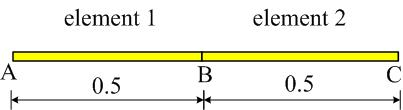
\includegraphics[width=7cm]{cable.jpg}    % The printed column width is 8.4 cm.
\caption{2 P1 elements}
\end{center}
\end{figure}

We use 2 P1 elements. See figure1.\\
 For element1, the shape functions are
\begin{equation}
\begin{cases}
\varphi_{A}^{(1)}=1-2x& \text{$\displaystyle 0 \leq x \leq 0.5$}\\
\varphi_{B}^{(1)}=2x& \text{$\displaystyle 0 \leq x \leq 0.5$}
\end{cases}
\end{equation}
 For element2, the shape functions are
\begin{equation}
\begin{cases}
\varphi_{A}^{(2)}=-2x+2& \text{$\displaystyle 0.5 < x \leq 1$}\\
\varphi_{B}^{(2)}=2x-1& \text{$\displaystyle 0.5 < x \leq 1$}
\end{cases}
\end{equation}
For element1, the stiffness matrix
\begin{gather*}
A^{(1)}=
\begin{pmatrix}
\int^{0.5}_{0}\varphi'^{(1)}_{A}\varphi'^{(1)}_{A}dx & \int^{0.5}_{0}\varphi'^{(1)}_{B}\varphi'^{(1)}_{A}dx\\
\int^{0.5}_{0}\varphi'^{(1)}_{A}\varphi'^{(1)}_{B}dx & \int^{0.5}_{0}\varphi'^{(1)}_{B}\varphi'^{(1)}_{B}dx
\end{pmatrix}=
\begin{pmatrix}
2 & -2\\
-2 & 2
\end{pmatrix}
\end{gather*}


\begin{gather*}
b^{(1)}=
\begin{pmatrix}
-0.25 \\
-0.25
\end{pmatrix}
\end{gather*}


For element2, the stiffness matrix
\begin{gather*}
A^{(2)}=
\begin{pmatrix}
2 & -2\\
-2 & 2
\end{pmatrix}, \qquad
b^{(2)}=
\begin{pmatrix}
-0.25 \\
-0.25
\end{pmatrix}
\end{gather*}



\begin{gather*}
A=
\begin{pmatrix}
2 & -2 &0\\
-2 & 4 & -2\\
0& -2 &2
\end{pmatrix}, \qquad
b=
\begin{pmatrix}
-0.25 \\
-0.5\\
-0.25
\end{pmatrix}
\end{gather*}
From the boundary condition, we know that $u_{A}=0$, the linear system change into
\begin{gather*}
\begin{pmatrix}
4 &-2\\
-2 &2
\end{pmatrix}
\begin{pmatrix}
u_{B} \\
u_{C}
\end{pmatrix}=
\begin{pmatrix}
-0.5\\
-0.25
\end{pmatrix}
\end{gather*}
\begin{gather*}
u_{B}= -0.375, \qquad u_{C}= -0.5.
\end{gather*}
\begin{equation}
\hat{u}=
\begin{cases}
-0.75x & \text{$\displaystyle 0\leq x \leq 0.5$}\\
-0.25x-0.25 & \text{$\displaystyle 0.5 <x \leq 1$}
\end{cases}
\end{equation}
The results are shown in Figure 2.

\begin{figure}[H]
\begin{center}
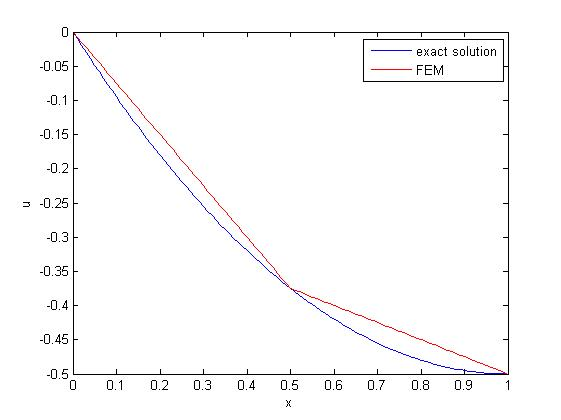
\includegraphics[width=8cm]{ex19.jpg}    % The printed column width is 8.4 cm.
\caption{Finite element approximation for $u''=1$ using 2 P1 elements}
\end{center}
\end{figure}

\end{document}

